\chapter{短文本主题模型的模型增强方法研究}\label{chap:sparentm}
\section{引言}
上一章提出了一种利用大规模语言模型的短文本扩充方法Instructed-Expansion,以及一种基于成对文本数据的主题模型TPTM。利用可以进行文本生成的LLMs,通过指令提示将每个短文本扩充为伪长文档,从而将LLMs的知识迁移到主题建模中。此外TPTM同时对短文本数据集和伪长文本数据集进行主题挖掘,假设短文本中的主题是从其对应伪文档中的主题中抽取的,以减轻文本生成过程中引入额外的主题信息对结果的影响。主题建模中潜在分布的参数估计是通过吉布斯采样来训练的。然而,我们也可以看到这种推理方式不够灵活,涉及大量的统计符号和公式推导,且对于大型语料库而言计算代价高昂。

近年来,深度学习的发展促使人们探索变分自编码器(VAE)\cite{VAE}来简化主题模型的推理过程 \cite{NVDM,AVITM},这一类利用神经网络搭建主题模型的方法称为神经主题模型\cite{NTMsurvey}(Neural Topic Models)。值得注意的是,使用狄利克雷分布是LDA模型成功让分布考虑平滑性和稀疏性的关键之一\cite{ZhaoPHJ}。狄利克雷变分自编码器模型(DVAE)\cite{DVAE}已成功地将狄利克雷先验约束施加于VAE网络中的表示层。然而,由于学习到的文档分布的稀疏性,VAE-LDA模型中狄利克雷先验的使用会对其挖掘出的潜在主题的质量造成影响\cite{overallQuality}。设置一个较小的狄利克雷先验值可以生成更稀疏的文档-主题分布,但这会迫使VAE将某些文档中存在的词汇分配一个几乎为零的概率,从而削弱其捕捉整个语义结构的能力\cite{DVAE,AVITM}。从而导致挖掘出的主题质量不佳的问题。因此,对文本稀疏结构的建模需要超越VAE-LDA模型中的狄利克雷先验的额外机制。上一章我们讨论了如何利用大规模语言模型增强短文本中的词共现信息。本章则聚焦于如何从模型增强的角度出发,构建一个增强稀疏表达的主题模型。

现有的工作往往修改了VAE-LDA模型中的网络架构以应对这一问题。例如批量归一化(Batch Normalization)和Dropout层被用来防止网络在训练过程中过分关注稀疏性\cite{Pachinko}。另一种方法是DVAE.Sp模型\cite{DVAE},它采用sigmoid激活函数来选择与每个文档相关的主题,旨在狄利克雷分布中解耦稀疏性和平滑性。然而,这些修改只影响训练过程,并没有将主题选择纳入主题模型的生成过程中。鉴于VAE-LDA模型中狄利克雷先验的局限性,将稀疏性考虑整合到LDA的生成过程中可能更为合适。

因此,本章在VAE-LDA框架中提出了一种新的稀疏增强的非均场主题模型(Sparsity Reinforced and Non-Mean-Field Topic Model,SpareNTM),包括两种创新的方法。首先,我们考虑一种除狄利克雷先验外的,辅助先验知识来进行稀疏性建模。在自编码框架中,一种可能的方式是使用Beta分布,如CRNTM模型\cite{CRNTM}所采用的先验,但这不能产生真正稀疏的表示。另一种方式是如TONOLINI和FALLAH等人\cite{VSC,VSCT,EVO_bi}在VAE中采用的“Spike and Slab”\cite{spike&slab}先验。但这些研究使用稀疏先验应用于图像生成领域。我们将这一想法纳入VAE-LDA模型中。因此,我们提出的SpareNTM使用二元潜变量来建模文档-主题分布中的稀疏性,即将伯努利先验引入到LDA的生成过程中。具体来说,SpareNTM为每个文档构建了一个使用伯努利变量的\textit{主题选择器},用以过滤掉不相关的主题。这样,每个文档的狄利克雷先验将被限制在所选主题的范围内。通过这种方式,我们的SpareNTM模型不仅维持了主题模型的解释性,还提高了其在处理文档集时的性能,尤其是在稀疏性较高的场景中。这种方法的关键优势在于它将稀疏性直接整合到模型的生成过程中,而不仅仅是作为训练过程中的一个调节因素。此外,通过引入二元潜变量,SpareNTM能够更有效地区分相关和不相关的主题,从而生成更加精确和一致的文档-主题分布。

其次,为了进行SpareNTM的推断步骤,我们设计了一个新颖的VAE网络,该网络采用非均场近似来估计真实后验。据我们所知,SpareNTM是首批使用非均场推理的神经主题模型之一。以往的神经主题模型\cite{CRNTM,TopicRNN,VRTM,SGTM}在引入VAE-LDA的辅助潜变量时,采用均场理论\cite{VI}对损失函数的推导过程进行简化。然而,TURNER和DREFS等人\cite{MFnegative,EVO}已经讨论了均场理论的负面影响,因为它未能解释潜变量之间的相关性。相反,我们的模型SpareNTM能够考虑到文档-主题分布与伯努利主题选择器在后验分布之间的关系。然后,我们应用“重参数化技巧”\cite{VAE}和Gumbel-Softmax估计器\cite{gumbel}来生成后验主题选择器。实验表明了我们方法在主题质量和稀疏性方面就有较大的优势。

本章的主要贡献可以总结如下:

(1)提出了一种神经主题模型,该模型使用伯努利先验对稀疏性进行建模,以获得主题质量与表示稀疏性之间的更好平衡。

(2)在VAE框架下开发了一个有效的网络结构来学习推理过程,该过程实现了后验近似中的非均场推理,以捕捉潜变量中的相关性。

(3)通过一系列实验,证明了SpareNTM在不同数据集上的主题质量和稀疏性方面优于现有模型。

\section{稀疏主题模型}
本节将描述我们提出的方法。本节首先会介绍SpareNTM的生成过程。接着提出了经过调整后的VAE主题模型,同时解释了非均场推理是如何应用的。最后详细介绍了模型对应的神经网络框架。

回顾前面章节给出的定义,给定一个包含$D$篇文本的语料库,其词汇$W$共有$V$个词汇,每篇文档$x$被处理成词袋(BOW)向量,形式为$x=[x_1,x_2,\dots,x_V]$,其中$x_i$代表第$i$个词在文档$x$中出现的次数。

% \subsection{VAE-LDA}
% 首先回顾VAE-LDA模型的框架。语料库中的每一篇文本$x$都可以被表示为在$K$个主题上,具有狄利克雷先验的一个文档-主题分布$\theta\sim Dir(\alpha)$。且主题-词分布$\beta_z$在词汇表$W$的$V$个词上对主题$z$进行建模。如果用$\beta$来表示矩阵$\beta=(\beta_1,\beta_2,\dots,\beta_K)^{T}$,文档中的词将独立同分布(i.i.d)地从分布$p(x\vert\theta;\beta)=\mbox{Multinomial}(1,\mbox{Softmax}(\theta^{T}\beta))$中抽取,被称为“product of experts”\cite{AVITM}。

% 将VAE应用于LDA模型时,模型会增加一个\textit{编码器}网络$f_{enc}$。具体来说,编码器将BOW $x$作为输入,并输出$\hat{\alpha}$,然后使用参数$\hat{\alpha}$的狄利克雷分布或其他分布$q(\theta|x;\hat{\alpha})$来近似真实的后验分布$p(\theta|x)$:
% \begin{align}
%     \hat{\alpha}:= f_{enc}(x;\Pi)\\
%     \tilde{\theta}\sim q(\theta|x;\hat{\alpha})\\
%     f_{dec}(\tilde{\theta};\beta):=\mbox{Softmax}(\tilde{\theta}^{T}\beta)
% \end{align}
% 在VAE框架下,通过最大化证据下界(ELBO)来优化编码器和解码器的参数:
% \begin{equation} 
%     \mathcal{L}(\Pi,\beta;x)=E_{q(\theta|x)}[\log p(x|\theta)]-KL(q(\theta\vert x;\hat{\alpha})\|p(\theta;\alpha))
% \end{equation}
% 在只采样一个样本的策略下\cite{VAE}, $E_{q(\theta|x)}[\log p(x|\theta)]\simeq x^{T}\log\ f_{dec}(\tilde{\theta})$.

\subsection{SpareNTM}
稀疏主题模型在传统主题模型的基础上引入稀疏假设(即每篇文档只和少量主题相关)。为了使得离散分布的采样过程能够得到有效的梯度计算以及反向传播,我们提出了稀疏增强的神经主题模型(Sparsity Reinforced Neural Topic Model, SpareNTM)。通过引入伯努利先验到文档-主题分布中,间接控制文档中的主题数量,将LDA模型与稀疏性相结合。简单来说,SpareNTM为每个主题构建一个伯努利变量,来决定该主题是否出现在当前文档中,因此每篇文档只关注少数几个主题。这样的设计可以直接在主题模型中引入稀疏性,使得每个文档的主题分布更加集中。在SpareNTM中,每个文档$d$被表示为一个包含$K$个主题的文档-主题分布$\theta\sim Dir(b_d\cdot\alpha)$,其中$b_d$是一个被称为主题选择器的向量。主题选择器$b_d=(b_{d1},…,b_{dK})$是一个长度为$K$的向量,由$K$个参数为$\lambda=(\lambda_1,\dots,\lambda_K)$的伯努利变量组成。因此,向量$b_d$鼓励文档$d$只关注一部分潜在的主题。当$b_d$的分量全为1时,SpareNTM将退化为标准的LDA模型。SpareNTM模型的生成过程如下:

\begin{enumerate}
	\item[(1)] 对于每一篇文档 $d \in \mathcal{D}$:
	\begin{enumerate}
		\item 对于主题选择器 $b_d$中的每一个分量:
		\begin{enumerate}
			\item 采样 $b_{d,k}\sim \mbox{Bernoulli}(\lambda_k)$
		\end{enumerate}
		\item 采样一个文档-主题分布 $\theta\sim \mbox{Dirichlet}(b\cdot\alpha)$
		\item 对于 $d$ 中的每个单词 $w_{n}$:
		\begin{enumerate}
			\item[] 采样一个单词实体 $w_n\sim \mbox{Multinomial}(1,\theta^{T}\beta)$
		\end{enumerate}
	\end{enumerate}
\end{enumerate}
因此,SpareNTM的编码器框架是:
\begin{align}
    \hat{\alpha},\hat{\lambda}:= f_{enc}(x;\Pi)\\
    \tilde{\theta}\sim q(\theta,b|x;\hat{\alpha},\hat{\lambda})\\
    f_{dec}(\tilde{\theta};\beta):=\mbox{Softmax}(\tilde{\theta}^{T}\beta) 
\end{align}

对于文档$d$,其联合概率密度函数为:
\begin{equation}
	\label{spLDA_joint}
	p(x,\theta,b\vert\alpha,\lambda,\beta)=p(b\vert\lambda)p(\theta\vert b;\alpha)\prod_{n=1}^{n_d} p(w_n\vert\theta;\beta)
\end{equation}
其中,假设$b$中每个分量都是独立的,有$p(b\vert\lambda)=\prod_{k=1}^{K}p(b_k\lambda_k)$。此外,可以从解码分布$p(w_n\vert\theta;\beta)=\mbox{Softmax}(\theta^T\beta)$中生成每个单词。

\subsection{目标函数}
基于上述伯努利先验的引入,我们假设一篇文章$x$对应的主题分布是$\theta$,及其伯努利主题筛选变量是$b$,其中1表示对应主题出现在该文本中,0则表示不含该主题。因此论文的目的是求得后验概率分布$p(\theta,b\vert x)$。由于此后验分布是不可求解的。在变分推断的框架下,需要推导一个变分分布$q(\theta,b|x;\hat{\alpha},\hat{\lambda})$以逼近这个后验分布。在本节中,论文为变分分布$q(\theta,b|x;\hat{\alpha},\hat{\lambda})$设计了一种基于神经网络的推断方法。传统的变分推断使用平均场理论,对潜变量之间的独立性做出强独立假设,以实现推断方法的可扩展性和易优化性\cite{VI}。以往的神经主题模型,如 TopicRNN \cite{TopicRNN}、CRNTM\cite{CRNTM}、VRTM\cite{VRTM}和SGTM\cite{SGTM},就采用平均场理论将辅助潜变量引入VAE-LDA时。然而,许多研究\cite{EVO,MFnegative}已经就无法解释潜变量之间的相关性讨论了许多关于平均场理论的负面影响。相比之下,我们定义了一个非均值场假设的变分分布Eq.(\ref{vq})来捕捉真实后验$p(\theta,b\vert x)$中$\theta$和$b$之间的相关性。
\begin{equation}
    q(\theta,b\vert x)=q(b\vert x;\hat{\lambda})q(\theta\vert x,b;\hat{\alpha})
    \label{vq}
\end{equation}
我们假设$q(b\vert x;\hat{\lambda})=\prod_{k=1}^{K}q(b_k\vert \hat{\lambda}_k)$,其中$q(b_k\vert \hat{\lambda}_k)$是具有概率$\hat{\lambda}_k$的伯努利分布。根据$p(\theta\vert b,\alpha)=\mbox{Dir}(b\cdot\alpha)$,类似地定义$q(\theta\vert x,b;\hat{\alpha})=\mbox{Dir}(b\cdot\hat{\alpha})$。在本章中,我们没有考虑$b_k$之间的依赖关系。这是因为目前我们希望模型能够捕捉到全局变量$\theta$和$b$之间的相互影响,这对于提高模型的表达能力而言更加重要。如前所述,狄利克雷分布在促进稀疏表示中也起着作用。因此,与仅依赖于二元潜变量(伯努利分布)作为先验的模型不同,$b\cdot\hat{\alpha}$有助于减轻忽略$b_k$之间依赖关系的负面影响。根据VAE-LDA模型的框架, 变分参数$\alpha$和$\hat{\lambda}=(\hat{\lambda}_1,\dots,\hat{\lambda}_K)$, 是编码器网络的输出。

通过推导变分推断背景下的证据下界(Evidence Lower Boubd,ELBO),可以优化这个非均值场的变分分布,以逼近真实的后验分布,从而提高模型在短文本主题建模中的性能和准确度。基于上述的定义,SpareNTM的证据下界(ELBO)由Eq.(\ref{myelbo})给出。这个目标可以被分解成如下形式:$\mathcal{L}=\mathcal{L}_{rec}+\mathcal{L}_\theta+\mathcal{L}_b$, where $\mathcal{L}_{rec}=E_{q(\theta,b\vert x)}\left[\log p(x\vert\theta)\right]$, $\mathcal{L}_\theta=-E_{q(\theta,b\vert x)}\left[\log\frac{q(\theta\vert x,b)}{p(\theta\vert b)}\right]$, and $\mathcal{L}_b=-E_{q(\theta,b\vert x)}\left[\log\frac{q(b\vert x)}{p(b)}\right]$。 我们的目标是最大化$\mathcal{L}$,以找到最佳的变分参数和模型参数。为了阐明ELBO所展示的内容,我们接下来详细讨论了ELBO中这三项期望的具体形式。
\begin{align}
    \label{myelbo}
    &\log(p(x,\theta,b\vert\alpha,\lambda,\beta))\geq\mathcal{L}(\Pi,\beta;x)=E_{q(\theta,b\vert x)}\left[\log p(x,\theta,b\vert \alpha,\lambda,\beta) - \log q(\theta,b\vert x)\right]\nonumber\\
	&=E_{q(\theta,b|x)}\left[\log p(x|\theta)\right]-E_{q(\theta,b|x)}\left[\log\frac{q(\theta|x,b)}{p(\theta|b)}\right]-E_{q(\theta,b|x)}\left[\log\frac{q(b|x)}{p(b)}\right]\nonumber\\
\end{align}

\textbf{(1)$\boldsymbol{\mathcal{L}_b}$}

对于$\mathcal{L}_b$,我们可以得到$\mathcal{L}_b=-\sum_{k=1}^{K}KL(q(b_k\vert x)\|p(b_k))$(推导细节见附录B.1),然后利用伯努利分布之间的KL散度计算得到解析表达式(\ref{kl2})。

\begin{equation}
    \label{kl2}
    KL(q(b_k\vert x;\hat{\lambda}_k)\|p(b_k;\lambda_k))=\hat{\lambda}_k\log\frac{\hat{\lambda}_k}{\lambda_k}+(1-\hat{\lambda}_k)\log\frac{1-\hat{\lambda}_k}{1-\lambda_k}
\end{equation}

\textbf{(2)$\boldsymbol{\mathcal{L}_\theta}$}

对于$\mathcal{L}_\theta$,我们可以得到$\mathcal{L}_\theta=-E_{q(b\vert x)}\left[KL(q(\theta\vert x,b)||p(\theta\vert b))\right]$(推导细节见附录B.2)。尽管此期望存在解析表达式,由于向量b的离散空间很大($2^K$),论文决定利用VAE中的重参数技巧\cite{VAE}处理这一表达式。通过Gumble-Softmax估计,可以从Bernoulli($\hat{\lambda}_k$)中采样得到$\tilde{b}_k,k=1,\dots,K$。因此$\mathcal{L}_{\theta}\approx-KL(q(\theta\vert x,\tilde{b})\|p(\theta\vert\tilde{b}))$,即利用狄利克雷分布之间的KL散度计算即可。

\begin{align}
	\label{kl1}
	&KL(q(\theta\vert x,\tilde{b})||p(\theta\vert \tilde{b}))=\log\Gamma(\sum_k\tilde{b}_k\cdot\hat{\alpha}_k)-\log\Gamma(\sum_k\tilde{b}_k\cdot\alpha_k)\nonumber+\sum_k\log\Gamma(\tilde{b}_k\cdot\alpha_k)\\
	&-\sum_k\log\Gamma(\tilde{b}_k\cdot\hat{\alpha}_k)+\sum_k\tilde{b}_k\cdot(\hat{\alpha}_k-\alpha_k)(\psi(\tilde{b}_k\cdot\hat{\alpha}_k)-\psi(\sum_k\tilde{b}_k\cdot\hat{\alpha}_k))
\end{align}

\textbf{(3)$\boldsymbol{\mathcal{L}_{rec}}$}

重构项是$\mathcal{L}{rec}=E_{q(\theta,b\vert x)}\left[\log p(x\vert\theta)\right]$。由于向量$b$已经在$\mathcal{L}_\theta$中被采样,并且变分分布是$q(\theta,b\vert x)=q(b\vert x)q(\theta\vert x,b)$,我们采用两步来从$q(\theta,b\vert x)$中采样$\theta$。首先,我们采样$\tilde{b}$,然后采样$\tilde{\theta}\sim\mbox{Dir}(\tilde{b}\cdot\hat{\alpha})$。因此,$\mathcal{L}{rec}$项可以近似为$\mathcal{L}{rec}\approx \log p(x\vert\tilde{\theta})=x^{T}\log\ f_{dec}(\tilde{\theta})$。

在应用SGVB(随机梯度变分贝叶斯)对变分下界(\ref{myelbo})进行优化后,现在可以重新给出模型的目标函数$\tilde{\mathcal{L}}\approx\mathcal{L}$,如下所示:
\begin{equation} 
	\begin{aligned}
		&\tilde{\mathcal{L}}(\Pi,\beta;x)=x^{T}\log\ f_{dec}(\tilde{\theta})-KL(q(\theta\vert x,\tilde{b})\|p(\theta\vert \tilde{b}))-\sum^K_{k=1}KL(q(b_k)\|p(b_k))\\
	\end{aligned}
	\label{elbo_approx}
\end{equation}
其中$\tilde{b}_k\sim\mbox{Bernoulli}(\hat{\lambda}_k)$,$k=1,2,\dots K$,且$\tilde{\theta}\sim\mbox{Dir}(\tilde{b}\cdot\hat{\alpha})$。 对于这个目标函数,我们可以明显地看出其与自编码器的联系。模型的编码器网络将文档词袋$x$映射到变分参数$\hat{\alpha}$和$\hat{\lambda}$,然后从相关分布中采样$\tilde{b}$和$\tilde{\theta}$。随后,解码器网络将$\tilde{\theta}$作为函数$\log p(x\vert\tilde{\theta})$的输入,该函数等于观测$x$的概率密度。解码器网络的目标是生成能够最大程度地重建原始观察值x的输出。网络的具体细节将在下一节中描述。

\subsection{网络框架}

完成了目标函数的推导之后,我们为其设计相应的变分自编码器网络框架。其中一个挑战是如何在VAE中实现对离散伯努利变量的采样。为了解决这个问题,我们采用类别自编码器的思想,并利用Gumbel-Softmax估计方法,以实现对伯努利变量的采样,并能够进行梯度反传优化。如图\ref{framework}所示,输入的文本$x$通过Relu激活函数以及dropout层进行线性变换。然后,上述变换的结果经过分支\ding{172},通过线性变换和批量归一化得到变分参数$\hat{\alpha}$。由于Dirichlet的参数不能为非正数,所以我们采用Softplus函数进行变换。分支\ding{173}进入主题选择模块,再次利用线性变换和批量归一化来得到$u_1$和$u_2$,分别代表主题是否被选中的比例。所以变分参数$\hat{\lambda}$(主题被选中的后验概率)是基于$u_1$和$u_2$的Softmax函数来计算的。现在可以用Gumbel-Softmax估计法从Bernoulli($\hat{\lambda}$)中对主题选择器$\tilde{b}$进行采样。对于主题第$k$个主题,定义$(\pi_{k1},\pi_{k2})=(\hat{\lambda}_k,1-\hat{\lambda}_k)$,有

\begin{equation}
	\tilde{b}_k=\frac{\exp{((\log(\pi_{k1})+g_1)/\tau})}{\sum_{i=1}^2\exp{((\log(\pi_{ki})+g_i)/\tau})}
\end{equation}
其中$g_1,g_2$是从Gumbel(0, 1)分布\footnote{Gumbel(0, 1)分布可以通过逆变换采样来抽样,方法是抽取$u\sim\mbox{Uniform(0, 1)}$,然后计算$g=-\log(-\log(u))$。}中独立同分布(i.i.d)抽样得到的,且$\tau$在实验中被设定为1。在生成主题选择器$\tilde{b}=(\tilde{b}_1,\dots,\tilde{b}_K)$之后,我们使用拒绝采样以及Gamma分布的增强采样方法\cite{DVAE,RSVI},采样稀疏的$\tilde{\theta}\sim\mbox{Dir}(\tilde{b}\cdot\hat{\alpha})$。

\begin{figure}[ht]
    \centering
    \includegraphics[trim=0cm 0.1cm 0cm 0.1cm, clip=false, width=0.65\textwidth]{chap4/network.pdf}
    \caption{SpareNTM的网络架构图} \label{framework}
\end{figure}


\section{实验设置}
\subsection{数据集}
模型的性能评估将在上一章介绍的三个短文本数据集上进行,同时增加两个常规文本对模型的鲁棒性进行评估,分别是20NewsGroups(20NG)和Wikitext-103(Wiki)\cite{wiki}。具体详情如下:
\begin{itemize}
\item \textbf{20NG} 包含大约18,000篇新闻文章,分为20个不同类别。
\item \textbf{Wiki} 是WikiText数据集的一个版本,包括来自Wikipedia的大约28,500篇文章。
\end{itemize}

对数据集进行同上一章对文本进行预处理的操作,移除了停用词以及长度等于1或出现频次少于100的单词。这两个数据集的基础信息在表\ref{corpus}中总结,其中$N$ 表示每个数据集中的文档数量,$L$ 显示每个文档的平均长度,$V$ 表示词汇表的大小。

\begin{table}
	\centering
	\caption{常规文本数据集的基本信息} \label{corpus}
	\adjustbox{width=0.35\textwidth}{
		\begin{tabular}{l|c|c|c}
			\hline
			数据集&$N$&$L$&$V$\\
			\hline
			20NG&18,846&87.5&2,000\\
                Wiki&28,532&133.4&20,000\\
			\hline
		\end{tabular}
	}
\end{table}

\subsection{对比模型}
本节将SpareNTM与LDA和以及多种不同的神经主题模型进行对比。对于常规主题模型,我们考虑了ProdLDA,DVAE。在考虑稀疏性的神经主题模型方面,我们将与DVAE.Sp,GSM,NSMDM \cite{SparseMax},SCHOLAR,和SBVAE进行比较。对于短文本数据集,我们还对比了NQTM \cite{NQTM}的效果。DVAE和SCHOLAR是最先进的神经主题模型,而NQTM在短文本中的表现优于传统主题建模。此外,我们还评估了SpareNTM-MF(使用均场假设的SpareNTM),以展示非均场推理的有效性。对比模型的详细介绍如下:

\textbf{(1)ProdLDA\cite{AVITM}:}该方法以拉普拉斯分布近似狄利克雷分布,以实现文档-主题分布在变分自编码器中的有效采样。

\textbf{(2)DVAE\cite{DVAE}:}该方法利用拒绝接受采样和伽马分布的增强采样方法,成功在变分自编码器总将狄利克雷分布作为文档-主题分布的先验分布。

\textbf{(3)DVAE.Sp\cite{DVAE}:}该方法是DVAE的稀疏化版本,其利用sigmoid激活函数构建了同我们一个目标的主题选择器变量。

\textbf{(4)GSM\cite{GSM}:}该方法利用高斯sotfmax构造( Gaussian Softmax Construction),在网络中强化隐变量的稀疏属性。

\textbf{(5)NSMDM\cite{SparseMax}:}该方法不同于GSM的稀疏构造,其采用sparsemax激活函数以进一步强化隐变量的稀疏属性。

\textbf{(6)SCHOLAR\cite{SCHOLAR}:}该方法是一种基于稀疏可加性生成模型的神经网络框架,灵活地结合了文档的元数据。

\textbf{(7)SBVAE\cite{SBVAE}:}该模型将狄利克雷过程中的Stick Breaking构造应用于变分自编码器,基于此开发了适用于主题建模的网络架构

\textbf{(8)NQTM\cite{NQTM}:}该模型基于VQ-VAE(Vector Quantised Variational AutoEncoder)构建了适用于短文本数据集的稀疏文档-主题分布。

\subsection{参数设置}
基线模型的网络结构和参数设置是根据其作者的指导构建和设置的。隐藏单元的数量设定为500,所有数据集使用200的批量大小。我们使用0.0001的学习率,并采用Adam优化器进行优化。

\section{实验结果与分析}

\subsection{与基线模型对比}
在本节中,我们将SpareNTM与基线模型进行比较。狄利克雷先验的值设置为0.02。对于SBVAE,stick-breaking先验和学习率分别设置为10和0.01。此外,对于20NG和Wiki,SpareNTM的伯努利先验设置为0.05,而在短文本数据集中设置为0.2。表\ref{Tweet topic quality},\ref{SearchSnippets topic quality}和\ref{StackOverflow topic quality}展示了在短文本数据集上,模型的NPMI指标、TU指标,以及整体主题质量TQ指标的结果。而表\ref{20News topic quality}和表\ref{Wiki topic quality}则展示了常规文本数据集上,模型的NPMI指标、TU指标和TQ指标的结果。对于每个模型,结果后的$\uparrow$或$\downarrow$表示根据5%显著性水平的t检验,该基准模型的表现显著优于或劣于我们提出的SpareNTM,并且最佳值以粗体标记。$K=50$和$K=100$的平均排名表示为av.rank。

\begin{table}
    \centering
    \caption{Tweet数据集在不同模型下的主题质量}
    \label{Tweet topic quality}
    \footnotesize
    \adjustbox{width=0.85\textwidth}{
    \begin{tabular}{cccc|cccc}
    \toprule
    \multirow{2}{*}{\textbf{Tweet}} & \multicolumn{3}{c}{K=25}&\multicolumn{3}{c}{K=50}&\\
    \cmidrule(lr){2-7}
    &NPMI&TU&\textbf{TQ}&NPMI&TU&\textbf{TQ}&av.rank\\
    \midrule
    LDA&0.187$\downarrow$ &0.872$\downarrow$ &0.163$\downarrow$ &0.184$\downarrow$ & 0.810 & 0.149$\downarrow$&3.5\\
    ProdLDA&0.181$\downarrow$&0.522$\downarrow$&0.094$\downarrow$&0.182$\downarrow$&0.415$\downarrow$&0.076$\downarrow$&10\\
    DVAE&0.179$\downarrow$&0.692$\downarrow$&0.124$\downarrow$&0.183$\downarrow$&0.426$\downarrow$&0.07$\downarrow$8&8.5\\
    DVAE.Sp&0.161$\downarrow$&0.820$\downarrow$ &0.132$\downarrow$ &0.148$\downarrow$ &0.730$\downarrow$ &0.108$\downarrow$ &6.5\\
    SBVAE&0.147$\downarrow$ &0.816$\downarrow$ &0.120$\downarrow$ &0.122$\downarrow$ &0.739$\downarrow$ &0.090$\downarrow$ &8.5\\
    GSM&0.172$\downarrow$&0.936$\downarrow$&0.161$\downarrow$&0.155$\downarrow$&0.779&0.121$\downarrow$&4.5\\
    NSMDM&0.178$\downarrow$&\textbf{0.953}&0.170$\downarrow$&0.173$\downarrow$&0.635$\downarrow$&0.110$\downarrow$&4.0\\
    SCHOLAR&0.174$\downarrow$ &0.845$\downarrow$ &0.147$\downarrow$ &0.171$\downarrow$ &0.621$\downarrow$ &0.106$\downarrow$ &6.5\\
    NQTM\cite{NQTM}&0.184$\downarrow$&\textbf{0.953}$\uparrow$&0.175$\downarrow$&0.180$\downarrow$&0.868$\uparrow$&0.156&2.0\\
    SpareNTM&\textbf{0.210} & 0.939 & \textbf{0.197} &\textbf{0.218} & 0.781 &\textbf{0.170} &1.0\\
    \bottomrule
\end{tabular}
}
\end{table}

\begin{table}
    \centering
    \caption{SearchSnippets数据集在不同模型下的主题质量}
    \label{SearchSnippets topic quality}
    \footnotesize
    \adjustbox{width=0.85\textwidth}{
    \begin{tabular}{cccc|cccc}
    \toprule
    \multirow{2}{*}{\textbf{SearchSnippets}} & \multicolumn{3}{c}{K=25}&\multicolumn{3}{c}{K=50}&\\
    \cmidrule(lr){2-7}
    &NPMI&TU&\textbf{TQ}&NPMI&TU&\textbf{TQ}&av.rank\\
    \midrule
    LDA&0.237$\downarrow$&0.804$\downarrow$&0.191$\downarrow$&0.225$\downarrow$ & 0.723$\downarrow$ & 0.163$\downarrow$&7.5\\
    ProdLDA&0.100$\downarrow$&0.709$\downarrow$&0.071$\downarrow$&0.094$\downarrow$&0.576$\downarrow$&0.054$\downarrow$&9.5\\
    DVAE&0.239$\downarrow$&0.915$\downarrow$&0.219$\downarrow$&0.246$\downarrow$&0.690$\downarrow$&0.170$\downarrow$&6.5\\
    DVAE.Sp&0.190$\downarrow$&0.868$\downarrow$&0.165$\downarrow$&0.172$\downarrow$&0.708$\downarrow$&0.122$\downarrow$&9.0\\
    SBVAE&0.230$\downarrow$&0.969$\downarrow$&0.223$\downarrow$&0.173$\downarrow$&0.702$\downarrow$&0.121$\downarrow$&7.5\\
    GSM&0.256$\downarrow$&0.968$\downarrow$&0.248$\downarrow$&0.236$\downarrow$&\textbf{0.960}&0.227$\downarrow$&2.0\\
    NSMDM&0.261$\downarrow$&0.947$\downarrow$&0.247$\downarrow$&0.214$\downarrow$&0.887$\downarrow$&0.190$\downarrow$&4.0\\
    SCHOLAR&0.253$\downarrow$&0.975$\downarrow$&0.247$\downarrow$&0.239$\downarrow$&0.863$\downarrow$&0.206$\downarrow$&3.5\\
    NQTM&0.245$\downarrow$&0.992&0.243$\downarrow$&0.238$\downarrow$&0.944&0.225$\downarrow$&4.0\\
    SpareNTM&\textbf{0.287} & \textbf{1.0} & \textbf{0.287} & \textbf{0.261} & 0.952 & \textbf{0.248}&1.0\\
    \bottomrule
\end{tabular}
}
\end{table}

\begin{table}
    \centering
    \caption{StackOverflow数据集在不同模型下的主题质量}
    \label{StackOverflow topic quality}
    \footnotesize
    \adjustbox{width=0.85\textwidth}{
    \begin{tabular}{cccc|cccc}
    \toprule
    \multirow{2}{*}{\textbf{StackOverflow}} & \multicolumn{3}{c}{K=25}&\multicolumn{3}{c}{K=50}&\\
    \cmidrule(lr){2-7}
    &NPMI&TU&\textbf{TQ}&NPMI&TU&\textbf{TQ}&av.rank\\
    \midrule
    LDA&\textbf{0.212}$\uparrow$ &0.592$\downarrow$ &0.126$\downarrow$ &\textbf{0.200} & 0.605$\downarrow$ & 0.121$\downarrow$&5.5\\
    ProdLDA&0.100$\downarrow$ &0.709$\downarrow$ &0.071$\downarrow$ &0.094$\downarrow$ &0.576$\downarrow$ &0.054$\downarrow$ &10\\
    DVAE&0.178$\downarrow$ &0.771$\downarrow$ &0.137$\downarrow$ &0.178$\downarrow$ &0.544$\downarrow$ &0.097$\downarrow$ &6.5\\
    DVAE.Sp&0.150$\downarrow$ &0.768$\downarrow$ &0.115$\downarrow$ &0.146$\downarrow$ &0.628$\downarrow$ &0.092$\downarrow$ &8.0\\
    SBVAE&0.123$\downarrow$ &0.797$\downarrow$ &0.098$\downarrow$ &0.117$\downarrow$ &0.637$\downarrow$ &0.075$\downarrow$ &9.0\\
    GSM&0.183$\downarrow$ &0.79$\downarrow$ &0.144$\downarrow$ &0.172$\downarrow$ &0.656$\downarrow$ &0.113$\downarrow$ &5.0\\
    NSMDM&0.182$\downarrow$ &\textbf{0.968}$\uparrow$ &0.176$\downarrow$ &0.170$\downarrow$ &\textbf{0.845}$\uparrow$ &0.144 &2.5\\
    SCHOLAR& 0.157$\downarrow$& 0.949&0.149$\downarrow$ & 0.14$\downarrow$& 0.732$\downarrow$&0.102$\downarrow$ &5.0\\
    NQTM&0.172$\downarrow$ & 0.957&0.164$\downarrow$ &0.176$\downarrow$ &0.844$\uparrow$ &{0.149} &2.0\\
    SpareNTM &0.203 & 0.943 & \textbf{0.191} & 0.190 & 0.785 & \textbf{0.149} &1.0\\
    \bottomrule
\end{tabular}
}
\end{table}

\textbf{(1)短文本数据集} 

从表\ref{Tweet topic quality},\ref{SearchSnippets topic quality}和\ref{StackOverflow topic quality}可以看到,SpareNTM主题质量上表现最佳。这再次证明,考虑稀疏性的模型比不考虑稀疏性的模型具有更好的主题质量。并且,由于短文本的稀疏特性,大多模型的在不同主题数量$K$下的表现不同,即模型受主题数量这一参数影响较大。所有模型在$K=50$时的主题质量都有所下降。此外,ProdLDA、DVAE.Sp和SBVAE在多数情况下的表现并不如LDA主题模型,这可能是因为这些模型的先验假设(如拉普拉斯近似狄利克雷分布,狄利克雷过程等)并在神经主题模型中并不适用。而考虑稀疏性的模型往往可以更好地挖掘出短文本中的潜在主题。尽管NQTM的表现仅次于SpareNTM,其使用离散自编码器在短文本建模中也具有天然优势,但其高内存要求使其不适用于常规文本数据集。简而言之,SpareNTM引入了额外的先验来建模稀疏性,通过非均值场的推断,同时利用了上一章提出的Instructed-Expansion方法,从而产生了较大的协同效应。
\newpage
\textbf{(2)常规文本数据集} 

从表\ref{20News topic quality}和表\ref{Wiki topic quality}可以观察到,在20NG数据集上,SpareNTM和NSMDM取得了最好的主题质量,其次是SCHOLAR和LDA。尽管在K=100时,NSMDM的表现略优于SpareNTM,但在K=50时,SpareNTM具有很大优势。在较长的Wiki数据集上,SpareNTM比其他模型表现得更好。论文提出的模型可以发现更有意义和更多样化的主题。与不考虑稀疏性的模型相比,其中DVAE具有最佳主题质量,SpareNTM表现出显著更好的主题质量。这表明狄利克雷先验优于其他先验假设。同时,作为DVAE的稀疏增强版本的SpareNTM证明了狄利克雷先验不足以满足稀疏建模的要求。考虑稀疏性的模型可以实现更好的主题质量。总之,我们发现SpareNTM相较其他模型而言,具有更广泛的适用性和鲁棒性,体现了其引入了额外的先验来建模稀疏性,且通过非均值场的推断的优越性。

\begin{table}
    \centering
    \caption{20News数据集在不同模型下的主题质量}
    \label{20News topic quality}
    \footnotesize
    \adjustbox{width=0.85\textwidth}{
    \begin{tabular}{cccc|cccc}
    \toprule
    \multirow{2}{*}{\textbf{20News}}& \multicolumn{3}{c}{K=50}&\multicolumn{3}{c}{K=100}&\\
    \cmidrule(lr){2-7}
    &NPMI&TU&\textbf{TQ}&NPMI&TU&\textbf{TQ}&av.rank\\
    \midrule
    LDA \cite{LDA}&0.248&0.580$\downarrow$&0.144$\downarrow$&0.249$\uparrow$&0.494$\downarrow$&0.123&3.5\\
    ProdLDA \cite{AVITM}&0.271$\uparrow$&0.475$\downarrow$&0.129$\downarrow$&0.250$\uparrow$&0.356$\downarrow$&0.089$\downarrow$&7.0\\
    DVAE \cite{DVAE}&\textbf{0.272}$\uparrow$&0.530$\downarrow$&0.144$\downarrow$&\textbf{0.262}$\uparrow$&0.385$\downarrow$&0.101$\downarrow$&5.0\\
    DVAE.Sp \cite{DVAE}&0.225$\downarrow$&0.525$\downarrow$&0.118$\downarrow$&0.218$\downarrow$&0.359$\downarrow$&0.078$\downarrow$&8.0\\
    SBVAE \cite{SBVAE}&0.171$\downarrow$&0.524$\downarrow$&0.090$\downarrow$&0.148$\downarrow$&0.363$\downarrow$&0.054$\downarrow$&9.0\\
    GSM \cite{GSM}&0.210$\downarrow$&0.644$\downarrow$&0.135$\downarrow$&0.200$\downarrow$&0.519$\downarrow$&0.104$\downarrow$&5.0\\
    NSMDM \cite{SparseMax}&0.222$\downarrow$&\textbf{0.784}&0.174$\downarrow$&0.200$\downarrow$&\textbf{0.651}$\uparrow$&\textbf{0.130}&1.5\\
    SCHOLAR \cite{SCHOLAR}&0.258$\uparrow$&0.603$\downarrow$&0.156$\downarrow$&0.239$\uparrow$&0.424$\downarrow$&0.101$\downarrow$&4.5\\
    SpareNTM&0.244&0.763&\textbf{0.186}&0.229&0.549&0.126&1.5\\
    \bottomrule
    \end{tabular}
    }
\end{table}

\begin{table}
    \centering
    \caption{Wiki数据集在不同模型下的主题质量}
    \label{Wiki topic quality}
    \footnotesize
    \adjustbox{width=0.85\textwidth}{
    \begin{tabular}{cccc|cccc}
    \toprule
    \multirow{2}{*}{\textbf{Wiki}} & \multicolumn{3}{c}{K=50}&\multicolumn{3}{c}{K=100}&\\
    \cmidrule(lr){2-7}
    &NPMI&TU&\textbf{TQ}&NPMI&TU&\textbf{TQ}&av.rank\\
    \midrule
    LDA&0.280$\downarrow$&0.617$\downarrow$&0.173$\downarrow$&0.286$\downarrow$&0.596$\downarrow$&0.170$\downarrow$&6.0\\
    ProdLDA&0.357$\downarrow$&0.471$\downarrow$&0.168$\downarrow$&0.377$\uparrow$&0.405$\downarrow$&0.153$\downarrow$&7.0\\
    DVAE&\textbf{0.403}&0.669$\downarrow$&0.270$\downarrow$&\textbf{0.396}$\uparrow$&0.491$\downarrow$&0.194$\downarrow$&5.0\\
    DVAE.Sp&0.197$\downarrow$&0.841$\downarrow$&0.166$\downarrow$&0.168$\downarrow$&0.701$\downarrow$&0.118$\downarrow$&9.5\\
    SBVAE&0.287$\downarrow$&0.967&0.278$\downarrow$&0.224$\downarrow$&0.580$\downarrow$&0.130$\downarrow$&6.5\\
    GSM&0.300$\downarrow$&0.974&0.292$\downarrow$&0.279$\downarrow$&\textbf{0.877}$\uparrow$&0.245$\downarrow$&3.5\\
    NSMDM&0.354$\downarrow$&\textbf{0.979}&0.347$\downarrow$&0.220$\downarrow$&0.625$\downarrow$&0.138$\downarrow$&5.0\\
    SCHOLAR&0.398&0.937$\downarrow$&0.373$\downarrow$&0.366&0.691$\downarrow$&0.253$\downarrow$&2.0\\
    SpareNTM&0.401&0.973&\textbf{0.390}&0.364&0.831&\textbf{0.302}&1.0\\
    \bottomrule
    \end{tabular}
    }
\end{table}

\subsection{消融实验} 
\textbf{(1)Instructed-Expansion数据增强的有效性}

为了评估Instructed-Expansion所得到的伪长文本对SpareNTM的影响,本节在原始短文本数据集和伪长文本数据集上分别运行SpareNTM进行比较,分别记为SpareNTM-short和SpareNTM-IE。表\ref{ablation1}展示了在这两种数据集上的运行结果。对于每个模型,结果后的$\uparrow$或$\downarrow$表示根据5%显著性水平的t检验,该基准模型的表现显著优于或劣于SpareNTM-IE可以看到Instructed-Expansion数据增强对短文本建模的提升效果是显著的。此外,尽管SpareNTM在原始短文本上的效果不如SpareNTM-IE,但与表\ref{Tweet topic quality},\ref{SearchSnippets topic quality}和\ref{StackOverflow topic quality}中的模型相比,也具有一定的竞争优势。

\begin{table}[ht]
    \centering
    \caption{原始短文本数据集和伪长文本数据集在SpareNTM下的结果。}
    \label{ablation1}
    \adjustbox{width=0.95\textwidth}{
    \begin{tabular}{lccc|ccc|ccc}
    \toprule
    \multicolumn{10}{c}{K=25}\\\hline
    \multicolumn{1}{c}{\multirow{2}{*}{模型}} & \multicolumn{3}{c|}{Tweet} & \multicolumn{3}{c|}{SearchSnippets} & \multicolumn{3}{c}{StackOverflow} \\
    \multicolumn{1}{c}{} & NPMI & TU & \textbf{TQ} & NPMI & TU & \textbf{TQ} & NPMI & TU & \textbf{TQ} \\\hline
    SpareNTM-short & 0.188$\downarrow$ &0.837$\downarrow$ &0.157$\downarrow$ & 0.230$\downarrow$&0.998&0.230$\downarrow$ & 0.176$\downarrow$ &0.973$\uparrow$ &0.167$\downarrow$  \\
    SpareNTM-IE & 0.210 & 0.939 & 0.197 & 0.287 & 1.0 & 0.287 & 0.203 & 0.943 & 0.191 \\\midrule
    \multicolumn{10}{c}{K=50}\\\hline
    \multicolumn{1}{c}{\multirow{2}{*}{模型}} & \multicolumn{3}{c|}{Tweet} & \multicolumn{3}{c|}{SearchSnippets} & \multicolumn{3}{c}{StackOverflow} \\
    \multicolumn{1}{c}{} & NPMI & TU & \textbf{TQ} & NPMI & TU & \textbf{TQ} & NPMI & TU & \textbf{TQ} \\\midrule
    SpareNTM-short & 0.180$\downarrow$ & 0.767$\downarrow$ & 0.138$\downarrow$ & 0.244$\downarrow$ & 0.978$\uparrow$ & 0.239$\downarrow$ & 0.157$\downarrow$ & 0.787 & 0.123$\downarrow$  \\
    SpareNTM-IE & 0.218 & 0.781 &0.170 & 0.261 & 0.952 & 0.248 & 0.190 & 0.785 & 0.149 \\
    \bottomrule
    \end{tabular}
    }
\end{table}

\textbf{(2)稀疏性与非均场推理方法的有效性}

为了评估将稀疏性纳入生成网络,以及SpareNTM中使用的非均场推理方法的有效性,表\ref{ablation2}将SpareNTM与,DVAE和SpareNTM-Mean-Field(SpareNTM-MF)进行比较。对于每个模型,结果后的$\uparrow$或$\downarrow$表示根据5%显著性水平的t检验,该基准模型的表现显著优于或劣于SpareNTM。尽管DVAE的NPMI得分会高于SpareNTM-MF,但在TU得分方面表现不佳。因此,在所有数据集中,SpareNTM-MF的主题质量均优于DVAE,这表明引入稀疏性增强了性能。此外,SpareNTM在它们中获得了最高的主题质量,特别是在TU得分方面,这表明了本章所提出方法的优越性,归功于在SpareNTM中应用的主题选择器和非均场推断方法。

\begin{table}
    \centering
    \caption{20News、Wiki 和 SearchSnippets分别在SpareNTM和SpareNTM-MF(使用均值场推断)下的结果}
    \label{ablation2}
    \adjustbox{width=0.95\textwidth}{
    \begin{tabular}{lccc|ccc|ccc}
    \toprule
    \multicolumn{1}{c}{\multirow{2}{*}{模型}} & \multicolumn{3}{c|}{20News} & \multicolumn{3}{c|}{Wiki} & \multicolumn{3}{c}{SearchSnippets} \\
    \multicolumn{1}{c}{} & NPMI & TU & \textbf{TQ} & NPMI & TU & \textbf{TQ} & NPMI & TU & \textbf{TQ} \\\midrule
    DVAE & 0.272$\uparrow$&0.530$\downarrow$&0.144$\downarrow$ & 0.403 & 0.669$\downarrow$ & 0.270$\downarrow$ & 0.190$\downarrow$&0.868$\downarrow$&0.165$\downarrow$ \\
    SpareNTM-MF & 0.236$\downarrow$&0.684$\downarrow$&0.161$\downarrow$ & 0.379$\downarrow$&0.940$\downarrow$&0.356$\downarrow$ & 0.214$\downarrow$ & 1.000$\uparrow$ & 0.214$\downarrow$  \\
    SpareNTM & 0.244 & 0.763 & 0.186 & 0.401 & 0.973 & 0.390 & 0.244 & 0.978 & 0.239 \\
    \bottomrule
    \end{tabular}
    }
\end{table}

\subsection{TPTM与SpareNTM的对比}
本节将SpareNTM与上一章提出的TPTM模型进行了对比。表\ref{TPTM vs SpareNTM}展示了SpareNTM和TPTM,在Tweet,SearchSnippets和StackOVerflow对应的IE-llama2数据集上的结果。对于每个模型,结果后的$\uparrow$或$\downarrow$表示根据5%显著性水平的t检验,该基准模型的表现显著优于或劣于SpareNTM。可以看到,TPTM在Tweet和StackOVerflow上的表现优于SpareNTM。一个可能的原因是Tweet数据集的样本量只有2,472,在神经网络模型中面对着样本数较少的问题,因此SpareNTM很难准确估计神经网络中的大量参数。对于StackOVerflow而言,则有可能是LLMs在获得其对应伪长文本的同时,引入了额外的主题的信息,因此TPTM更适用于此类伪文档的主题挖掘。而在SearchSnippets数据集上,SpareNTM的表现要全面优于TPTM。总之,如同Qiang\cite{STTM}等人的研究证明,没有任何一个短文本主题模型能在所有的短文本数据集上达到最优。

\begin{table}[ht]
    \centering
    \caption{K=50时,TPTM与SpareNTM在三个伪长文本数据集上的结果}
    \label{TPTM vs SpareNTM}
    \adjustbox{width=0.95\textwidth}{
    \begin{tabular}{lccc|ccc|ccc}
    \toprule
    \multicolumn{1}{c}{\multirow{2}{*}{模型}} & \multicolumn{3}{c|}{Tweet} & \multicolumn{3}{c|}{SearchSnippets} & \multicolumn{3}{c}{StackOverflow} \\
    \multicolumn{1}{c}{} & NPMI & TU & \textbf{TQ} & NPMI & TU & \textbf{TQ} & NPMI & TU & \textbf{TQ} \\\midrule
    TPTM-llama2 & 0.225 & 0.871$\uparrow$ & 0.196$\uparrow$ & 0.241$\downarrow$ & 0.874$\downarrow$ & 0.211$\downarrow$ & 0.218$\uparrow$ & 0.773 & 0.169$\uparrow$\\
    SpareNTM & 0.218 & 0.781 &0.170 & 0.261 & 0.952 & 0.248 & 0.190 & 0.785 & 0.149 \\
    \bottomrule
    \end{tabular}
    }
\end{table}

\subsection{参数影响实验}
在本节,我们首先研究了伯努利先验$\lambda$的影响。我们选择在20NG数据集上运行SpareNTM,并将狄利克雷先验$\alpha$设为0.02。表\ref{selected topics}展示了在不同$\lambda$值下,在测试集数据上计算得到的平均主题数量。可以观察到,当增加$\lambda$的取值时,SpareNTM找到的平均主题数量也随之增长,并且几乎遵循二项分布$E[\mbox{B}(K,\lambda)]=\lambda\cdot K$的期望值,而DVAE.Sp只能永远固定选择$K$个主题的一半。因此,通过结合伯努利先验,SpareNTM可以灵活地强制每篇文档专注于$K$个主题的一小部分。

图\ref{Performance_Bern}展示了在不同$\lambda$值和$K=50$条件下SpareNTM的NPMI和TU得分。可以观察到NPMI在0.230到0.250的小范围内变化,这表明本章在LDA模型中考虑稀疏性以挖掘语义信息这一方法是稳定的。相比之下,当$\lambda$增大时,TU得分下降,并在$\lambda=0.05$时获得最佳值。此时每篇文档平均选择了3个主题,这个数量小于参数设置中的主题数量$K$,甚至小于20NG中实际类别的数量。这是因为每篇文档专注于少数几个主题的假设是合理的。

\begin{table}[ht]
    \centering
    \caption{在20NG上,不同$\lambda$下,SpareNTM选择的平均主题数与DVAE.Sp进行对比} 
    \label{selected topics}
    \adjustbox{width=0.65\textwidth}{
        \begin{tabular}{c|ccccc|cc|ccc}
            \toprule
            \multicolumn{1}{c}{}&\multicolumn{7}{c}{SpareNTM}&\multicolumn{3}{c}{DVAE.Sp}\\
            \midrule
            K&\multicolumn{5}{c}{50}&100&200&50&100&200\\
            \midrule
            $\lambda$&0.2&0.4&0.5&0.6&0.8&0.1&0.1&-&-&-\\
            \midrule
            Avg.num&10&21&27&31&41&11&20&25&46&102\\
            \bottomrule
        \end{tabular}
    }
\end{table}

\begin{figure}
    \centering
        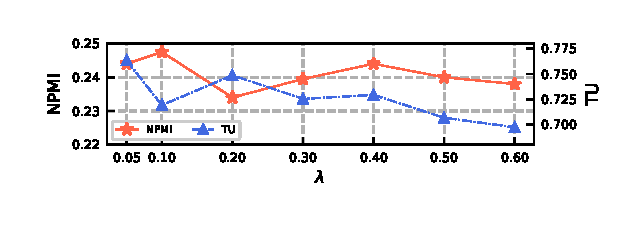
\includegraphics[trim=0.3cm 0.4cm 0.25cm 0.3cm, clip=true, width=0.8\textwidth]{chap4/Bernoulli.eps}
        \caption{在20NG数据集上,K=50时,SpareNTM在不同Bernoulli先验$\lambda$值下的NPMI和TU} \label{Performance_Bern}
\end{figure}


\begin{figure}
    \centering
        \includegraphics[trim=0.4cm 0.4cm 0.3cm 0.3cm, clip=false, width=\textwidth]{chap4/document_topic.pdf}
        \caption{当K=50时,20NG数据集中某个随机文本的文档-主题表示。以子图(h)为例,反应出该文本在只关注50个主题中的4个主题,以及在这4个主题上的概率大小。} \label{document_topic_figure}
\end{figure}
\subsection{文档-主题分布示例}
\textbf{(1)文档-主题表示示例}

本节从20NG数据集中随机选择了一篇与宗教相关的文档,并在K=50的情况下分析了不同模型生成的文档-主题表示。图\ref{document_topic_figure}中每个子图的y轴代表主题$T=[1,2,\dots,50]$,而x轴对应于主题概率。图\ref{document_topic_figure}清楚地展示了SpareNTM生成了更清晰的文档表示,这归功于其能够捕捉到每篇文档中更精确的语义信息。虽然一些基线模型也可以产生稀疏的主题分布,但我们提出的模型在稀疏的主题分布下实现了更好的主题质量。

\textbf{(2)主题示例评估} 

为了定性地展示SpareNTM生成的高质量主题,表\ref{topic examples}展示了在20NG数据集中与宗教相关的主题词,这些词是由LDA、DVAE、NSMDM、SCHOLAR和SpareNTM生成的。此外,表\ref{topic examples}将图\ref{document_topic_figure}中每个主题分布对应的两个概率最高的主题加粗显示。其他模型倾向于生成重复的主题,其中包含重复的单词。LDA和NSMDM则将不相关的主题分配给文档。相比之下,SpareNTM生成了与相关主题一致且多样化的主题。

\begin{table}[ht]
	\centering
	\caption{不同模型生成的与宗教相关的主题}
	\label{topic examples}
	\footnotesize
	\adjustbox{width=0.65\textwidth}{
		\begin{tabular}{ll}
			\toprule
            模型&\multicolumn{1}{c}{与宗教相关的主题}\\
            \midrule
            LDA&\makecell{\textbf{god believe truth one evidence}\\god jesus christian church christ\\\textbf{writes system morality keith organization}}\\
            \midrule
            DVAE&\makecell{\textbf{god Christians gods faith bible}\\jesus god bible christ faith\\heaven christ jesus sin lord\\\textbf{god Christians bible christ sin}\\morality objective evidence moral definition}\\
            \midrule
            NSMDM&\makecell{\textbf{christians biblical holy jesus sin}\\god gods faith atheist heaven\\morality objective absolute values mac\\\textbf{constitution government catholic amendment moral}}\\
            \midrule
            SCHOLAR&\makecell{god belief faith existence evidence\\god bible jesus christians christian\\christian christians god christ church\\\textbf{jesus christ church faith christians}\\\textbf{morality moral keith objective definition}}\\
            \midrule
            SpareNTM&\makecell{\textbf{jesus sin christians christ bible}\\ christ mary lord jesus heaven\\existence atheist belief islam exist\\\textbf{morality objective moral values keith}}\\
            \bottomrule
            \end{tabular}
        }
\end{table}


\section{本章小结}

本章提出了一种带有辅助伯努利变量的SpareNTM主题模型,以更好地建模文本潜在语义结构的稀疏性,并开发了一个有效的VAE网络来学习推理过程。所提出的方法可以通过识别哪些主题出现在文档中,从而发现文档-主题的稀疏性,在主题质量和泛化能力方面均优于现有方法。在多个语料库上的实验结果表明,我们的模型获得了比其他方法更高的NPMI得分和更多样化的主题。在未来的工作中,计划在在SpareNTM中考虑伯努利潜变量的相互影响时的影响。
